\section{Packet Filter Firewall}
\label{sec:packet-filter-firewall}

Werden verschiedene Computernetzwerke miteinander verbunden, entstehen unweigerlich Sicherheitsrisiken. In einem Netzverbund ist es nicht immer wünschenswert, dass Besucher aus einem (fremden) Netz Zugriff auf alle Ressourcen im eigenen Netz erhalten.

Mit der \emph{Packet Filter Firewall} kann ein- und ausgehender IP-basierter Datenverkehr analysiert und mit entsprechenden Regeln gefiltert werden.


\subsection*{Kontext}
Das eigene Computernetzwerk wird mit verschiedensten anderen Netzen verbunden. Jedes dieser Netze besitzt unterschiedliche ``Levels of Trust''.

Als kleinsten gemeinsamen Nenner läuft jegliche Kommunikation in diesen Netzen über das Internet Protocol (IP). Die dadurch entstehenden Datenpakete können aufgrund der Informationen in deren Header analysiert werden.

\subsection*{Problem}
Hosts in fremden Netzen sind potentielle Angreifer auf Ressourcen in unserem Netz. Gibt es eine Möglichkeit, diese Hosts zu erkennen und den von ihnen ausgehenden Netzwerkverkehr bestmöglich zu blockieren?

Folgende Faktoren spielen dabei eine wichtige Rolle:

\begin{itemize}
	\item Eine komplette Abschottung des eigenen Netzes ist keine Option: Kommunikation ist ein wichtiger Bestandteil des ``Daily Business''.
	\item Für den Benutzer soll die Sicherheitsmassnahme transparent sein und keinen zusätzlichen Aufwand bedeuten (Login etc.)
	\item Der umzusetzende Mechanismus soll flexibel auf Änderungen anpassbar sein und die organisatorischen Sicherheitsrichtlinien so präzis wie möglich abbilden.
	\item Die Lösung soll so wenig Leistung wie möglich benötigen
\end{itemize}


\subsection*{Lösung}

Die \emph{Packet Filter Firewall} analysiert ein- und ausgehenden Netzwerkverkehr. Dabei wird jedes einzelne IP-Paket auf den Inhalt in seinem Header betrachtet und mit einem Set von definierten Regeln geprüft.

Diese Regeln bestehen im Normalfall aus einer Kombination von Ports und IP-Adressen oder IP-Adress-Bereichen. Dabei kann eine Regel sowohl Zugriff gewähren als auch verbieten.

Auf diese Weise können sehr komplexe Sicherheitsdispositive gebildet und geprüft werden. Um aber auch bei komplexeren Regelsets eine optimale Performance zu erzielen ist die Reihenfolge der Regeln von grösster Bedeutung.

\subsubsection*{Beispiel: Prüfung eingehendes IP-Paket}

\begin{enumerate}
	\item Ein fremder Host möchte auf eine Ressource im eigenen Netz zugreifen.
	\item Die \emph{Packet Filter Firewall} sucht anhand der Quell-IP-Adresse sowie des Ziel-IP-Adresse und -Ports nach einer passenden Regel
	\item Wird eine passende Regel gefunden, wird das Paket entsprechend zugelassen (oder verworfen, falls die Regel dies so definiert)
	\item Wird keine passende Regel gefunden, kommt eine Standard-Regel zum Zuge. Möchte man hohe Sicherheit gewährleisten, besagt diese meistens, dass das Paket verworfen werden soll.
\end{enumerate}

\begin{figure}[H]
	\centering
	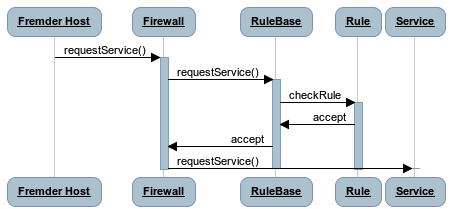
\includegraphics[width=12cm]{content/firewall-architectures/images/packet-filter-firewall-sequence.png}
	\caption{Packet Filter Firewall Sequenzdiagramm}
\end{figure}

Der Akteur \emph{RuleBase} bietet minimale Verwaltungsfunktionen (\gls{CRUD}) für Firewall-Regeln.


\subsection*{Vorteile}
\begin{itemize}
	\item Die Firewall filter für den Benutzer transparent jeglichen Netzwerkverkehr
	\item Da die Firewall jedes IP-Paket beim empfangen oder senden einmal ``in den Händen'' hat, ermöglicht die Firewall ein ausführliches Logging an den Schnittstellen zwischen verschiedenen Netzwerken.
	\item Eine \emph{Packet Filter Firewall} verschlingt minimale Ressourcen/Leistung. Unter anderem da lediglich die strukturierten Header-Informationen eines IP-Pakets analysiert werden.
\end{itemize}

\subsection*{Nachteile}
\begin{itemize}
	\item Fälscht ein potentieller Angreifer seine IP-Adresse, kann dies die \emph{Packet Filter Firewall} nicht erkennen und versagt in dieser Situation.
	\item Die Leistungsfähigkeit der Firewall ist stark von der Reihenfolge der definierten Regeln abhängig. Beispiel: Möchte man einen kompletten IP-Adress-Bereich blockieren, macht es wenig Sinn, diesen am Ende der Regelliste zu platzieren und so alle feingranularen Regeln zuerst zu prüfen.
	\item Die \emph{Packet Filter Firewall} kann keine Attacken auf Layern über IP erkennen. Da nur IP-Headers analysiert werden, können im IP-Payload problemlos schädliche Befehle/schädlicher Code enthalten sein.
	\item Natürlich kann die Firewall nur erfolgreich Netzwerkverkehr analysieren, welcher auch über diese geleitet wird. Es gilt also sicherzustellen, dass alle Wege in das zu schützende Netz über die Firewall(s) geleitet werden (\nameref{sec:singleaccesspoint})
\end{itemize}

\subsection*{Reallife Beispiele}
\begin{itemize}
	\item In einem Landwirtschaftsbetrieb ist jedes Tier (Netzwerkverkehr) mit einem RFID (IP-Header) ausgestattet. Will ein Tier in den Stall (zu schützendes Netz), wird es durch eine Schleuse (Firewall) geleitet. Anhand der Informationen auf dem RFID gelangt das Tier in den Stall, falls der Bauer dies vorneweg so erlaubt (Regeldefinition) hat. Darf das Tier den Stall nicht betreten, wird es wieder ins Freie geleitet.
\end{itemize}

\subsection*{Mögliche Prüfungsfragen}
\begin{itemize}
	\item \emph{Was ist ausschlaggebend für die Performance einer (Packet Filter) Firewall?}\\
	Die Optimierung der Reihenfolge der Firewall-Regeln.
	\item \emph{Wie erreichen Sie ein Höchstmass an Sicherheit mit der Verwendung einer (Packet Filter) Firewall?}\\
	Jeglicher Netzwerkverkehr muss über die Firewall geleitet werden. Weiter wird die Standardregel für Behandlung von eingehendem Netzwerkverkehr so eingestellt, dass dieser verboten wird. Anschliessend müssen nur noch Regeln für den erlaubten Verkehr erstellt werden.
\end{itemize}